


\documentclass[12pt,a4paper]{report}


\usepackage[utf8]{inputenc}
\usepackage{amsmath}
\usepackage{amsfonts}
\usepackage{amssymb}
\usepackage{graphicx}
\usepackage{amsthm}
\usepackage{natbib}
\usepackage{algorithm}
\usepackage{algpseudocode}

\usepackage{hyperref}
\AtBeginDocument{\let\textlabel\label}

\usepackage{marginnote}
\renewcommand*{\marginfont}{\scriptsize }







\theoremstyle{plain}
\newtheorem{thm}{Theorem}
\newtheorem{lemma}{Lemma}
\newtheorem{prop}{Proposition}

\theoremstyle{definition}
\newtheorem{definition}{Definition}
\newtheorem{remark}{Remark}
\newtheorem{example}{Example}


% Custom commands

\newcommand{\naive}{na\"{\i}ve }
\newcommand{\Naive}{Na\"{\i}ve }
\newcommand{\andor}{and\textbackslash or }
\newcommand{\erdos}{Erd\H{o}s }
\newcommand{\renyi}{R\`enyi }


\newcommand{\al}{\alpha}
\newcommand{\be}{\beta}

\newcommand{\set}[1]{\left\{ #1 \right\}} % A set
\newcommand{\rv}[1]{\mathbf{#1}} % A random variable
\newcommand{\x}{\rv x} % The random variable x 
\newcommand{\y}{\rv y} % The random variable y
\newcommand{\expect}[1]{\mathbf{E}\left[ #1 \right]} % The expectation operator
\newcommand{\expectg}[2]{\mathbf{E}_{\rv{#1}}\left[ \rv{#2} \right]} % An expectation w.r.t. a particular random variable.
\newcommand{\expectn}[1]{\mathbb{E}\left[#1\right]} % The empirical expectation
\newcommand{\cov}[1]{\mathbf{C}ov \left[ #1 \right]} % The expectation operator
\newcommand{\covn}[1]{\mathbb{C}ov \left[ #1 \right]} % The expectation operator
\newcommand{\gauss}[1]{\mathcal{N}\left(#1\right)} % The gaussian distribution
\newcommand{\cdf}[2]{F_\rv{#1} (#2)} % The CDF function
\newcommand{\cdfn}[2]{\mathbb{F}_{#1}(#2)} % The empirical CDF function
\newcommand{\icdf}[2]{F_\rv{#1}^{-1} (#2)} % The invecrse CDF function
\newcommand{\icdfn}[2]{\mathbb{F}^{-1}_{#1}(#2)} % The inverse empirical CDF function
\newcommand{\pdf}{p} % The probability density function
\newcommand{\dist}{P} % The proabaiblity distribution
\newcommand{\entropy}{H}
\newcommand{\mutual}{I}

\newcommand{\estim}[1]{\widehat{#1}} % An estimator

\newcommand{\norm}[1]{\Vert #1 \Vert} % The norm operator
\newcommand{\normII}[1]{\norm{#1}_2} % The norm operator
\newcommand{\normI}[1]{\norm{#1}_1} % The norm operator
\newcommand{\lik}{\mathcal{L}} % The likelihood function
\newcommand{\loglik}{L} % The log likelihood function
\newcommand{\loss}{l} % A loss function
\newcommand{\risk}{R} % The risk function
\newcommand{\riskn}{\mathbb{R}} % The empirical risk
\newcommand{\deriv}[2]{\frac{\partial #1}{\partial #2}} % A derivative
\newcommand{\argmin}[2]{argmin_{#1}\set{#2}} % The argmin operator
\newcommand{\argmax}[2]{argmax_{#1}\set{#2}} % The argmin operator
\newcommand{\hyp}{f} % A hypothesis
\newcommand{\hypclass}{\mathcal{F}} % A hypothesis class
\newcommand{\hilbert}{\mathcal{H}}
\newcommand{\rkhs}{\hilbert_\kernel} % A hypothesis class
\newcommand{\normrkhs}[1]{\norm{#1}_{\rkhs}}

\newcommand{\plane}{\mathbb{L}} % A hypoerplane
\newcommand{\categories}{\mathcal{G}} % The categories set.
\newcommand{\positive}[1]{\left[ #1 \right]_+} % The positive part function
\newcommand{\kernel}{\mathcal{K}} % A kernel function
\newcommand{\featureS}{\mathcal{X}} % The feature space
\newcommand{\indicator}[1]{I_{\set{#1}}} % The indicator function.
\newcommand{\reals}{\mathbb{R}}



\newcommand{\latent}{S}
\newcommand{\loadings}{A}
\newcommand{\rotation}{R}
\newcommand{\similaritys}{\mathfrak{S}}
\newcommand{\similarity}{s} % A similarity measure.
\newcommand{\dissimilarity}{d} % A similarity measure.
\newcommand{\dissimilaritys}{\mathfrak{D}}
\newcommand{\scalar}[2]{\left< #1,#2 \right>}



\newcommand{\manifold}{\mathcal{M}} % A manifold.
\newcommand{\project}{\hookrightarrow} % The orthogonal projection operator.
\newcommand{\projectMat}{H} % A projection matrix.
\newcommand{\rank}{q} % A subspace rank.
\newcommand{\encode}{E}
\newcommand{\decode}{D}


\newcommand{\ensembleSize}{M} % Size of a hypothesis ensemble.
\newcommand{\ensembleInd}{m} % Index of a hypothesis in an ensemble.


\newcommand{\sample}{\mathcal{S}} % A data sample.
\newcommand{\test}{\risk(\hyp)} % The test error (risk)
\newcommand{\train}{\riskn(\hyp)} % The train error (empirical risk)
\newcommand{\insample}{\bar{\risk}(\hyp)} % The in-sample test error.
\newcommand{\EPE}{\risk(\hat{\hyp}_n)} % The out-of-sample test error.
\newcommand{\folds}{K} % Cross validation folds 
\newcommand{\fold}{k} % Index of a fold
\newcommand{\bootstraps}{B} % Bootstrap samples
\newcommand{\bootstrap}{{b^*}} % Index of a bootstrap replication




\author{Jonathan Rosenblatt}
\title{Class Notes (experimental)}




\begin{document}

\maketitle

This text draws from \cite{hastie_elements_2003} and \cite{shalev-shwartz_understanding_2014}.
The former is freely available online.
For a softer introduction, with more hands-on examples, see \cite{james_introduction_2013}, also freely available online.
All books are very well written and strongly recommended.

The notation conventions used in this text have been collected in Appendix \ref{sec:notation}.


\tableofcontents

\newpage





\section{Estimation}
\label{sec:estimation} 
In this section, we present several estimation principles. 
Their properties are not discussed, as the section is merely a reminder and a preparation for what follows.
These concepts and examples can be found in many introductory books to statistics. I particularly recommend \cite{wasserman_all_2004} or \cite{abramovich_statistical_2013}.

\subsection{Moment matching}
\label{sec:moment_matching}

The fundamental idea: match empirical moments to theoretical. I.e., estimate
$$ \expect{g(X)}   $$
by 
$$ \expectn{g(X)}   $$
where $\expectn{g(x)}:=\frac{1}{n}  \sum_i g(x_i)$, is the empirical mean.

\begin{example}[Exponential Rate]

Estimate $\lambda$ in $\x_i \sim exp(\lambda)$, $i=1,\dots,n$, i.i.d.
$\expect{x}=1/\lambda$.
$\Rightarrow \estim{\lambda}=1/\expectn{x}$ .

\end{example}


\begin{example}[Linear Regression]

Estimate $\be$ in $\y \sim \gauss{X\be,\sigma^2 I}$, a $p$ dimensional random vector.
$\expect{y}=X\be$ and $\expectn{y}=y$.
Clearly, moment matching won't work because no $\be$ satisfies $X\be=y$.
A technical workaround:
Since $\be$ is $p$ dimensional, I need to find some $g(\y): \mathbb{R}^n \mapsto \mathbb{R}^p$.
Well, $g(y):=Xy$ is such a mapping. I will use it, even though my technical justification is currently unsatisfactory. We thus have:
$\expect{X'y}=X'X\be$ which I match to $\expectn{X'y}=X'y$:
$$
  X'X \be = X' y \Rightarrow \estim{\be}=(X'X)^{-1} X'y.
$$

\end{example}


\subsection{Quantile matching}
\label{sec:quantiles}

The fundamental idea: match empirical quantiles to theoretical. 
Denoting by $\cdf{x}{t}$ the CDF of $\x$, then $\icdf x \al$ is the $\al$ quantile of $\x$.
Also denoting by $\cdfn x t$ the Empirical CDF of $x_1,\dots, x_n$, then $\icdfn x \al$ is the $\al$ quantile of $x_1,\dots, x_n$.
The quantile matching method thus implies estimating
$$ \icdf x \al $$
by 
$$ \icdfn x \al  . $$

\begin{example}[Exponential rate]
Estimate $\lambda$ in $\x_i \sim exp(\lambda)$, $i=1,\dots,n$, i.i.d.
\begin{align*}
	& \cdf x t = 1-\exp(-\lambda t) = \al \Rightarrow \\
	& \icdf x \al = \frac{-\log(1-\al)}{\lambda} \Rightarrow \\
	& \icdf{x}{0.5} = \frac{-\log(0.5)}{\lambda} \Rightarrow \\
	& \estim{\lambda} = \frac{-\log(0.5)}{\icdfn{x}{0.5}}.
\end{align*}

\end{example}


\subsection{Maximum Likelihood}
\label{sec:ml}

The fundamental idea is that if the data generating process (i.e., the \emph{sampling distribution}) can be assumed, then the observations are probably some high probability instance of this process, and not a low probability event:
Let $\x_1,\dots,\x_n \sim P_\theta$, with density (or probability) $p_\theta(x_1,\dots,x_n)$.
Denote the likelihood, as a function of $\theta$: $\lik(\theta): p_\theta(x_1,\dots,x_n)$.
Then $$\estim{\theta}_{ML}:= argmax_{\theta}\set{ \lik(\theta) }.$$

Using a monotone mapping such as the log, does not change the $argmax$. 
Denote $$\loglik(\theta):=\log(\lik(\theta)).$$

 
\begin{example}[Exponential rate]

Estimate $\lambda$ in $X_i \sim exp(\lambda)$, $i=1,\dots,n$, i.i.d.
Using the exponential PDF and the i.i.d. assumption
$$ \lik(\lambda) = \lambda^n \exp(-\lambda \sum_i X_i), $$
and 
$$ \loglik(\lambda) = n \log(\lambda) -\lambda \sum_i X_i. $$

By differentiating and equating $0$, we get $\estim{\lambda}_{ML}=1/\expectn{X}$.

\end{example}

\begin{example}[Discrete time Markov Chain]

Estimate the transition probabilities,  $p_1$ and $p_2$ in a two state, $\set{0,1}$, discrete time, Markov chain where:
$P(\x_{t+1}=1|x_{t}=0)=p_1$ and $P(\x_{t+1}=1|X_{t}=1)=p_2$.
The likelihood:
$$
  \lik(p_1,p_2)=
  P(X_2,\dots,X_T;X_1,p_1,p_2)=
  \prod_{t=1}^T P(X_{t+1}=x_{t+1}|X_{t}=x_t).
$$
We denote $n_{ij}$ the total number of observed transitions from $i$ to $j$ and get that $\estim{p}_1=\frac{n_{01}}{n_{01}+n_{00}}$, and that $\estim{p}_2=\frac{n_{11}}{n_{11}+n_{10}}$.

\begin{remark}[Confession]
Well, this is a rather artificial example, as because of the Markov property, and the stationarity of the process, we only need to look at transition events, themselves Bernoulli distributed. 
This example does show, however, the power of the ML method to deal with non i.i.d. samples. As does the next example.
\end{remark}
\end{example}




\begin{example}[Autoregression of order 1 (AR(1))]
Estimate the drift parameter $a$,  in a discrete time Gaussian process where:
$\x_{t+1}=a \x_t+ \varepsilon; \varepsilon \sim \gauss{0,\sigma^2} \Rightarrow \x_{t+1}|\x_t \sim \gauss{a x_t,\sigma^2}$.

We start with the conditional density at time $t+1$:
$$
  p_{\x_{t+1}|\x_t=x_t}(x_{t+1}) = 
  (2 \pi \sigma^2)^{-1/2} \exp \left( 
    -\frac{1}{2 \sigma^2}(x_{t+1}-a x_t)^2 
  \right).
$$
Moving to the likelihood:
$$
  \lik(a) = 
  (2 \pi \sigma^2)^{-T/2} \exp \left(
    -\frac{1}{2 \sigma^2}\sum_{t=1}^T (x_{t+1}-a x_t)^2 
  \right).
$$
Taking the log and differentiating with respect to $a$ and equating $0$ we get $\estim{a}_{ML}=\frac{\sum x_{t+1}x_{t}}{\sum x_t^2}$.

We again see the power of the ML device.
Could we have arrived to this estimator by intuiton alone? Hmmmm... maybe. 
See that $Cov[X_{t+1},X_t] = a \; Var[X_t] \Rightarrow a=\frac{Cov[X_{t+1},X_t]}{Var[X_t]}$.
So $a$ can also be derived using the moment matching method which is probably more intuitive.

\end{example}




\begin{example}[Linear Regression]

Estimate $\be$ in $Y \sim \gauss{X\be,\sigma^2 I}$, a $p$ dimensional random vector.
Recalling the multivariate Gaussian PDF:
$$
  p_{\mu,\Sigma}(y) = 
  (2 \pi)^{-n/2} |\Sigma|^{-1/2} \exp\left(
    -\frac{1}{2} (y-\mu)' \Sigma^{-1} (y-\mu)
  \right)
$$
So in the regression setup:
$$
  \lik(\be)= 
  p_{\be,\sigma^2}(y) = 
  (2 \pi)^{-n/2} |\sigma^2 I|^{-1/2} \exp\left(
    -\frac{1}{2 \sigma^2} \normII{y-X\be}^2
  \right)
$$
and $\estim{\be}_{ML}$ equals 
\begin{align}
	\estim{\be}_{ML}=(X'X)^{-1} X'y.
\end{align}


\end{example}


\subsection{M-Estimation and Empirical Risk Minimization}
\label{sec:m_estimation}

M-Estimation, know as Empirical Risk Minimizaton (ERM) in the machine learning literature, is a very wide framework which stems from statistical desicion theory.
The underlying idea is that each realization of $\x$ incurs some loss, and we seek to find a "policy", in this case a parameter, $\theta^*$ that minimizes the average loss.
In the econometric literature, we dot not incur a loss, but rather a utility, we thus seek a policy that maximizes the average utility.

\begin{definition}[Loss Function]
The penalty for predicting $\theta$ when observing $x$: 
\begin{align}
	\loss(x;\theta).
\end{align}

\end{definition}
\begin{definition}[Risk Function]
The expected loss: 
\begin{align}
	\risk(\theta):=\expect{\loss(\x;\theta)}.
\end{align}

\end{definition}
Then the best prediction, $\theta^*$, being the minimizer of the expected risk is
\begin{align}
\label{eq:risk_min}
 \theta^*:= \argmin{\theta}{\risk(\theta)}.
\end{align}

As we do not know the distribution of $\x$, we cannot solve Eq.(\ref{eq:risk_min}), so we minimize the \emph{empirical} risk.
\begin{definition}[Empirical Risk]
The average loss in the sample: 
\begin{align}
	\riskn(\theta):=\expectn{\loss(x;\theta)}=\frac{1}{n}\sum_i \loss(x_i,\theta).
\end{align}
\end{definition}

A prediction that can actually be computed with data is thus the empirical minimizer $\estim{\theta}$:
\begin{align}
\label{eq:empirical_risk_min}
 \estim{\theta}:= \argmin{\theta}{\riskn(\theta)}.
\end{align}



\begin{example}[Squared Loss]
\label{eg:squared_loss}

Let $\loss(x;\theta)=(x-\theta)^2$. Then 
$
	\risk(\theta) = 
	\expect{(\x-\theta)^2} = 
	(\expect{\x}-\theta)^2 + Var[\x]. 
$
Clearly  $Var[\x]$ does not depend on $\theta$  so that $\risk(\theta)$ is minimized by $\theta^*=\expect{\x}$.
\textbf{We thus say that the expectation of a random variable is the minimizer of the squared loss.}

How do we estimate the population expectation? Well a natural estimator is the empirical mean, which is also the minimizer of the empirical risk $\riskn(x)$. The proof is immediate by differentiating. 
\end{example}


\begin{example}[Ordinary Least Squares (OLS)]
\label{eg:OLS}
Define the loss $\loss(y,x;\be):=\frac{1}{2}(y-x\be)^2$.
Computing the risk, $\expect{\frac{1}{2} \normII{\y-\x\be}^2}$ will require dealing with the joint distribution of $(\x,\y)$.
We don't really care about that right now. 
We merely want to see that the empirical risk minimizer, is actually the classical OLS problem. 
And well, it is (by definition actually):
\begin{align*}
	\riskn(\be)=\sum_{i=1}^n 	\frac{1}{2}(y_i-x_i\be)^2 = \frac{1}{2}\normII{y-x\be}^2.
\end{align*}
Minimization is easiest with vector derivatives, but I will stick to regular derivatives:
\begin{align*}
	\deriv{\riskn(\be)}{{\be_j}} = \sum_i \left[ (y_i-\sum_{j=1}^p x_{ij}\be_j)(-x_{ij}) \right]
\end{align*}
Equating $0$ yields $\estim{\be_j}=\frac{\sum_i y_i x_{ij}}{\sum_i x_{ij}^2}$.
Solving for all $j$'s and putting in matrix notation we get
\begin{align}
	\estim{\be}_{OLS}=(X'X)^{-1} X'y.
\end{align}

\end{example}


\subsection{Notes}

\subsubsection{Maximum Likelihood} 
Maximum likelihood estimators are a particular instance of M-estimators, if we set the loss function to be the negative log likelihood of the (true) sampling distribution.


\subsubsection{Choosing the Loss Function}
While by far the most popular, we do not automatically revert to minimizing a squared error loss.
There are several considerations when choosing the loss function.
Most ERM learning methods can be applied with different loss functions. 

The first consideration is computational complexity: if you choose a loss function that leads to a non-convex empirical risk, you are in trouble. There are no guarantees you will be able to find the risk minimizer in finite computing time.

The second consideration is the nature of the outcome $y$. Some loss functions are more appropriate to continuous $y$'s and some for categorical $y$'s. Typical loss functions for continuous $y$'s are the squared loss, absolute loss, and hinge loss.
Typical loss functions for categorical $y$'s are the Binomial likelihood loss (also known as the Cross Entropy, or Deviance), and the hinge loss. 

A third consideration, which is rarely given the importance it should get, is ``What is the meaning of $\theta^*$''? Or, ``What are we actually estimating''?
As we have seen in Example~\ref{eg:squared_loss}, the squared loss implies we are aiming to estimate the population mean.
What are we estimating when we use the hinge loss? The binomial loss? 
We will not discuss these matters, as we are discussing methods where these choices have already been made for us. 
When the day you start thinking of your own learning algorithms, you will need to give some thought to this question.



\section{From Estimation to Supervised Learning}
\label{sec:learning}

\subsection{Empirical Risk Minimization (ERM) and Inductive Bias}
In Supervised Learning, or \emph{learning with teacher},  we want to extract the relation $y=\hyp(x)$ between attributes $x$ and some outcome $y$.
It is implicit, and essential, that the outcomes are observed. If this is not the case, see \emph{Unsupervised Learning }(\S\ref{sec:unsupervised}).
The attributes, also know as \emph{features}, or \emph{predictors}, are assumed to belong to some \emph{feature space} $\featureS$. \marginnote{Feature Space}

Unlike classical statistics, we don't care to explain the causal process relating $x$ and $y$, we just want good predictions.  The implied ERM problem is
\begin{align}
	\estim{\hyp}(x) := \argmin{\hyp}{\riskn(\hyp(x))} = \argmin{\hyp}{\frac{1}{n} \sum_i \loss(y_i - \hyp(x_i))}.
\end{align}
Alas, there are clearly infinitely many $\hyp$ for which $\riskn(\estim{\hyp}(x))=0$, in particular, all those where $\estim{\hyp}(x_i)=y_i, \forall i$.
All these $\hyp$ feel like very bad predictors, as they \emph{overfit} the observed data, at a cost of generalizability.\marginnote{Overfitting}
We formalize this intuition in Section~\ref{sec:desicion_theory}. 

We need to make sure that we do not learn overly complex predictors, which generalize poorly to new data.
Motivated by the fact that humans approach new problems equipped with their past experience, this regularization is called \emph{Inductive Bias}. \marginnote{Inductive Bias}
There are several ways to introduce this bias, which can be combined:
\begin{description}
\item[Constrained Hypothesis Classes]
We typically do not allow $\hyp$ to be ``any function'' but rather restrict it to belong to a certain class. In the machine learning terminology, $\hyp$ is a Hypothesis, and it belongs to $\hypclass$ which is the Hypothesis Class.\marginnote{Hypothesis}
\item[Regularization] We do not need to treat all $\hyp \in \hypclass$ equivalently. We might have prior preferences towards particular $\hyp$'s , typically simple $\hyp$'s, and we can introduce these preferences in the learning process. This is called \emph{Regularization}.\marginnote{Regularization}
\item[Non ERM Approaches] Many learning problems can be cast as ERM problems, but another way to introduce bias is by learning $\hyp$ in a non-optimal manner. Inductive bias is thus introduced by the (non) optimization algorithm 
Learning algorithms that cannot be cast as ERMs include: Nearest Neighbour (\S\ref{sec:knn}), Kernel Regression(\S\ref{sec:kernel}), Boosting (\S\ref{sec:boosting}).
\end{description}

We now proceed to show that many supervised learning algorithms are in fact ERMs with some type of inductive bias: constrained hypothesis class \andor or regularization \andor suboptimality.

\subsection{Ordinary Least Squares (OLS)}
\label{sec:ols}
As seen in Example~\ref{eg:OLS}, by adopting a squared error loss, and restricting $\hypclass$ by assuming $\hyp$ is a linear function of $x$, we get the OLS problem.
In this case learning $\hyp$ is effectively the same as learning $\be$ as they are isomorphic, as will be the case in all hypothesis classes that admit a finite dimensional parametrization.

\paragraph{Regularization}
While the OLS problem seemingly has no regularization parameters, we are in no way restricted to the original $X$ matrix supplied to us. 
We are free to choose any subset of the $X$ variables. Selecting a subset of the $X$ variables is known as \emph{model selection}.\marginnote{Model Selection}
We will discuss many different methods to choose the regularization level, in this case, the variables in the OLS, in Section~\ref{sec:desicion_theory}.

We are not only free to select a subset of $X$s, but we can also augment $X$ with new variables, consisting of non linear transformation of the original ones. This is know as \emph{basis augmentation}. \marginnote{Basis Augmentation}
The idea of basis augmentation is a useful and fundamental one that will revisit us throughout the course, even if we typically don't call it by its name.

\begin{remark}[No Sampling Distribution]
We emphasize, that unlike the classical statistical literature, we never assumed any sampling distribution. 
This is why we will not be doing hypothesis testing on the model parameters.
ERM can be thus seen as \emph{exploratory} statistics. 

In particular, we are not discussing hypothesis testing and confidence intervals for the OLS problem, for this same reason: because we are not assuming the data generating distribution. This, in contrast to the classical statistical literature where the linear model is both the data generating process, and the assume hypothesis class. 

In statistical terminology, we may be fitting \emph{misspecified models}, we simply do not care about it, as long as predictions are good. \marginnote{Misspecified Model}
\end{remark}


\begin{remark}[OLS Extensions]
Most if not all extensions of OLS, such as Generalized Least Squared (GLS) and Generalized Linear Models (\S\ref{sec:logistic}) are ERM problems. 
\end{remark}




\subsection{Ridge Regression}
\label{sec:ridge}

Consider the Ridge regression problem:
\begin{align}
\label{eq:ridge}
	& \argmin{\be}{\frac{1}{n}\sum_i (y_i-x_i\be)^2 + \frac{\lambda}{2}\normII{\be}^2} \\
	& \estim{\be}_{Ridge}= (X'X+\lambda I)^{-1} X'y
\end{align}
We can see that again, $\hypclass$ is restricted to be the space of linear functions of $x$, but we also add a regularization that favours linear functions with small coefficients.

The regularization of $\be$ can have several interpretations and justifications:
\begin{description}
\item[A mathematical device] Strengthening the diagonal of $X'X$ makes is more easily invertible. This is a standard tool in applied mathematics called \emph{Tikhonov Regularization}. It is also helpful when dealing with multicolinearity, as $(X'X+\lambda I)$ is always invertible.
\item[A Subjective Bayesian View] If we believe that $\be$ should be small; say our beliefs can be quantified by $\rv \be \sim \gauss{0,1/\lambda I}$, then the Ridge solution is actually the mean of our posterior beliefs on $\rv \be|y$.
\end{description}

Whatever justification you prefer, it can be easily shown that $\deriv{\risk(\lambda,\be)}{\lambda}$ at $\lambda=0$ is negative, thus, predictions only improve by introducing some small regularization (how small is small? See \S\ref{sec:desicion_theory}).

For more on Ridge regression see \cite{hastie_elements_2003}.


\subsection{LASSO}
\label{sec:lasso}

Consider the LASSO problem:
\begin{align}
\label{eq:lasso}
	& \argmin{\be}{\frac{1}{n}\sum_i (y_i-x_i\be)^2 + \lambda \normI{\be}} 
\end{align}
As can be seen, just like in Ridge regression, $\hypclass$ is restricted to linear functions of $x$. The regularization however differs. Instead of $l_2$ norm penalty, we use an $l_1$ norm penalty.
Eq.(\ref{eq:lasso}) does not have a closed form solution for $\estim{\be}_{LASSO}$ but the LARS algorithm, a quadratic programming algorithm, solves it efficiently.



The LASSO has gained much popularity as it has the property that $\estim{\be}_{LASSO}$ has many zero entries. It is thus said to be \emph{sparse}\marginnote{Sparsity}.
The sparsity property is very attractive as it acts as a model selection method, allowing to consider $X$s where $p>n$, and making predictions computationally efficient.

The sparsity property can be demonstrated analytically for the orthogonal design case ($X'X=I$), in which $\estim{\be}$ admits a closed form solution:
\begin{align}
	\estim{\be}_{j,LASSO} = sign(\estim{\be}_{j,OLS}) \left[|\estim{\be}_{j,OLS}|-\frac{\lambda}{2} \right]_+.
\end{align}
We thus see that the LASSO actually performs \emph{soft thresholding} on the OLS estimates. \marginnote{Soft Thresholding}




\subsection{Logistic Regression}
\label{sec:logistic}
The logistic regression is the first categorical prediction problem we consider. \marginnote{Categorical Prediction}
I.e., the outcome $y$ is not a continuous variable, but rather takes values in some finite set $\categories$. In the logistic regression problem, it can take two possible values.
In the statistical literature, $y$ is encoded as $\categories=\set{0,1}$ and $\hyp$ is assumed to take to take the following form:
\begin{align}
	& p(x):= P(\y=1|x) = \Psi(x\be) \\
	& \Psi(t) = \frac{1}{1+e^{-t}}
\end{align}
The hypothesis class is thus  $\hypclass=\set{\hyp:\hyp(x)=\Psi(x\be)} $.

In the $\set{0,1}$ encoding, the loss is the negative log likelihood, i.e.:
\begin{align}
	\loss(y,x,\be) = 
	-\log \left[ p(x)^{y} (1-p(x))^{1-y}  \right] =
	-\log \left[ \Psi(x\be)^{y} (1-\Psi(x\be))^{1-y}  \right].
\end{align}
In the learning literature it is more common for $\categories=\set{1,-1}$ encoding of $y$ in which case the loss is 
\begin{align}
	\loss(y,x,\be) = -\log \left[ 1+\exp(-y f(x))  \right].
\end{align}


\paragraph{How to classify?}
In the $\set{0,1}$ encoding, we predict class $1$ if $\Psi(x\be)>0.5$ and class $0$ otherwise.
The logistic problem thus defines a separating hyperplane $\plane \subset \featureS$ between the classes: $\plane=\set{x:f(x)=0.5}$.

In the $\set{1,-1}$ encoding, we predict class $1$ if $\Psi(x\be)>0$ and class $0$ otherwise.
The plane $\plane$ is clearly invariant to the encoding of $y$.




\begin{remark}[Generalized Linear Models (GLM)]
Logistic regression is a particular instance of the very developped theory of Generalized Linear Models.\marginnote{GLM}
These models include the OLS, Probit Regression, Poisson Regression, Quasi Likelihood, Multinomial Regression, Proportional Odds regression and more.
The ultimate reference on the matter is \cite{mccullagh_generalized_1989}.
\end{remark}




\subsection{Regression Classifier}
\label{sec:regression_classifier}
Can we use the OLS framework for prediction? Yes! With proper encoding of $y$.
Solving the same problem from Example~\ref{eg:OLS} by encoding $y$ as $\set{0,1}$ gives us the linear separating hyperplane $\plane= \set{x:x\estim{\be}_{OLS}=0.5}$.

\begin{remark}
We can interpret $\estim{y}$ as the probability of an event, but there a slight technical difficulty as $\estim{y}$ might actually be smaller than $0$ or larger than $1$.
\end{remark}




\subsection{Linear Support Vector Machines (SVM)}
\label{sec:svm}

The literature typically presents the SVM method using the geometrical arguments that originally motivated the problem. 
For our purposes, we present the ERM formulation of the problem, followed by the original arguments.
Assuming a linear hypothesis class, $\hyp(x)=\be_0+\be x$, and $\categories=\set{-1,1}$ encoding, the SVM ERM problem is

\begin{align}
\label{eq:svc_ERM}
	\min_{\be,\be_0} \set{
		\sum_i \positive{1-y_i \hyp(x_i)} +\frac{\lambda}{2} \normII{\be}^2
	}.
\end{align}
Eq.(\ref{eq:svc_ERM}) thus reveals that the linear SVM is actually an ERM problem, over a linear hypothesis class, with what is called the \emph{hinge} loss function and $l_2$ regularization of $\be$.


\subsubsection{Geometrical Motivation for SVM}
For completeness, we present Vapnik's original geometric motivation \citep{vapnik_statistical_1998} for the formulation of the SVM problem. 

We do not assume anything on the data, and seek for a hyperplane $\plane$ that seperates two classes. 
Encode $y$ as $\categories=\set{-1,1}$.
Define a plane $\plane=\set{x: \hyp(x)=0 }$, and assume a linear hypothesis class, $\hyp(x)=x\be+\be_0$.
Now find the plane $\plane$ that maximizes the (sum of) distances to the data points.
We call the minimal distance from $\plane$ to the data points, the \emph{Margin}, and denote it by $M$.

To state the optimization problem, we need to note that $\hyp(x)=x\be+\be_0$ is not only the value of our classifier, but it is actually proportional to the signed distance of $x$ from $\plane$. 
\begin{proof}
The distance of $x$ to $\plane$ is defined as $\min_{x_0 \in \plane} \set{ \normII{x-x_0} }$.
Note $\be^*:=\be/\normII{\be}$ is a normal vector to $\plane$, since $\plane=\set{x: x\be+\be_0=0 }$, so that for $x_1,x_2 \in \plane \Rightarrow \be(x_1-x_2)=0$.
Now $x-x_0$ is orthogonal to $\plane$ because $x_0$ is, by definition, the orthogonal projection of $x$ onto $\plane$.
Since $x-x_0$ are both orthogonal to $\plane$, they are linearly dependent, so that by the Cauchy Schwarz inequality $\normII{\be^*} \normII{x-x_0}= \normII{\be^*(x-x_0)}$.
Now recalling that $\normII{\be^*}=1$ and $\be^* x_0=-\be_0/\normII{\be}$ we have $\normII{x-x_0}=\frac{1}{\normII{\be}} (x\be+\be_0)= \frac{1}{\normII{\be}} \hyp(x)$.
\end{proof}

Using this fact, then $y_i \hyp(x_i)$ is the distance from $\plane$ to point $i$, positive for correct classifications and negative for incorrect classification. 
The (linear) support vector classifier is defined as the solution to
\begin{align}
\label{eq:svc_separable}
	\max_{\be,\be_0} \set{ 
		M \quad s.t. \quad 
		\forall i: y_i \hyp(x_i) \geq M, \quad \normII{\be}=1
	}
\end{align}

If the data is not separable by a plane, which is typically the case, we need to allow some slack.
We thus replace $y_i \hyp(x_i) \geq M$ with $y_i \hyp(x_i) \geq M(1-\xi_i)$, for $\xi_i>0$ but require that the missclassifications are controlled using a regularization parameter $C$: $\sum_i \xi_i \leq C$.
Eq.(\ref{eq:svc_separable}) now becomes \citep[Eq.(12.25)]{hastie_elements_2003}
\begin{align}
\label{eq:svc_non_separable}
	\max_{\be,\be_0} \set{ 
		M \quad s.t. \quad 
		\forall i: y_i \hyp(x_i) \geq M(1-\xi_i), 
		\: \normII{\be}=1, 
		\: \sum_i \xi_i \leq C,
		\:\forall i:\xi_i\ \geq 0
	}
\end{align}


See Section 12 in \cite{hastie_elements_2003} for more details on SVMs.


\begin{remark}[Name Origins]
SVM takes its name from the fact that $\estim{\be}_{SVM}=\sum_i \estim{\al}_i y_i x_i$.
The explicit form of $\estim{\al}_i$ can be found in \citep[Section 12.2.1]{hastie_elements_2003}.
For our purpose, it suffices to note that $\estim{\al}_i$ will be $0$ for all data points far away from $\plane$.
The data points for which $\estim{\al}_i>0$ are the \emph{support vectors}, which give the method its name.
\end{remark}





\begin{remark}[Solve the right problem]
Comparing with the logistic regression, and the linear classifier, we see that the SVM cares only about the decision boundary $\plane$. Indeed, if only interested in \emph{predictions}, estimating \emph{probabilities} is a needless complication. As Put by Vapnik: 
\begin{quote}
When solving a given problem, try to avoid a more general problem as an intermediate
step.
\end{quote}
Then again, if the assumed logistic model of the logistic regression, is actually a good approximation of reality, then it will outperform the SVM as it borrows information from all of the data, and not only the support vectors. 
\end{remark}


\subsection{Generalized Additive Models (GAMs)}
\label{sec:gam}
A way to allow for a more broad hypothesis calss $\hypclass$, that is still not too broad, so that overfitting is hopefully under control, is by allowing the predictor to be an additive combination of simple functions.
We thus allow $\hyp(x)=\be_0 + \sum_{j=1}^p f_j(x_j)$. We also not assume the exact form of $\set{f_j}_{j=1}^p$ but rather learn them from the data, while constraining them to take some simple form.
The ERM problem of GAMs is thus
\begin{align}
\label{eq:GAM}
	 \argmin{\hyp \in \hypclass}{\frac{1}{n}\sum_i (y_i-\hyp(x_i))^2  }
\end{align}
where $\hyp$ is as defined above.

\begin{remark}[Not a pure ERM]
The learning of $\set{f_j}_{j=1}^p$ is in fact not performed by optimization, but rather by kernel smoothing (\S~\ref{sec:kernel}).
The solution to Eq.(\ref{eq:GAM}) is not a pure ERM problem, but a hybrid between ERM and kernel smoothing.
\end{remark}



\subsection{Projection Pursuit Regression (PPR)}
\label{sec:ppr}
Another way to generalize the hypothesis class $\hypclass$, which generalizes the GAM model, is to allow $\hyp$ to be some simple function of a linear combination of the predictors. Let 
\begin{align}
\label{eq:PPR}
	\hyp(x)=\sum_{m=1}^M g_m(w_m x)
\end{align}
where both $\set{g_m}_{m=1}^M$ and $\set{w_m}_{m=1}^M$ are learned from the data. 
The regularization is now performed by choosing $M$ and the class of $\set{g_m}_{m=1}^M$.
The ERM problem is the same as in Eq.(\ref{eq:GAM}), with the appropriate $\hyp$.

\begin{remark}[Not a pure ERM]
Just like the GAM problem, in the PPR problem $\set{g_m}_{m=1}^M$ are learned by Kernel Regresson (\S\ref{sec:kernel}). Solving the PPR problem is thus a hybrid of ERM and Kernel Regresson algorithms.
\end{remark}

\begin{remark}[Universal Approximator]
By choosing a sufficiently large $M$, the class $\hypclass$ can approximate any continuous function. This property of the class is called a \emph{Universal Approximator}.\marginnote{Universal Approximator}
\end{remark}




\subsection{Neural Networks (NNETs)}
\subsubsection{Single Hidden Layer}
In the spirit of \cite[Section 11]{hastie_elements_2003}, we introduce the NNET model via the PPR model, and not through its historically original construction.
In the language of Eq.(\ref{eq:PPR}), a \emph{single-layer--feed-forward }neural network, is a model where $\set{g_m}_{m=1}^M$  are not learned from the data, but rather assumed a-priori. 
\begin{align*}
	g_m(x):= \be_m \sigma( x \al_m  )
\end{align*}
where only $\set{\be_m, \al_m}_{m=1}^M$ are learned from the data. 
A typical \emph{activation function}\marginnote{Activation Function}, $\sigma(t)$ is the standard logistic CDF: $\sigma(t)=\frac{1}{1+e^{-t}}$. Another popular alternative are Gaussian radial functions.

As can be seen, the NNET is merely a non-linear regression model.
The parameters of which are often called \emph{weights}.

NNETs have gained tremendous popularity, as they strike a good balance between model complexity and regularity; particularly in the machine vision, sound analysis and natural language processing domains, where data samples are abundant.

\paragraph{Loss Functions}
Like any other ERM problem, we are free to choose the appropriate loss function.
For regression the squared loss is used. For classification, one can still use the squared error (as in the Regression Classifier), or the binomial likelihood leading to what is know as the \emph{deviance}, or \emph{cross-entropy} loss.\marginnote{Deviance \& Cross Entropy}

\paragraph{Universal Approximator}
Like the PPR, even when $\set{g_m}_{m=1}^M$ are fixed beforehand, the class is still a universal approximator (although it might require a larger $M$ than PPR).

\paragraph{Regularization}
Regularization of the model is done via the selection of the $\sigma$, the number of nodes/variables in the network and the number of layers. More that one hidden layer leads to \emph{Deep Neural Networks} which offer even more flexibility at the cost of complexity, thus requiring many data samples for fitting.\marginnote{Deep Neural Networks}

\paragraph{Back Propagation}
The fitting of such models is done via a coordinate-wise gradient descent algorithm called \emph{back propagation}.

\paragraph{Further Reading}
For more on NNETs see \citep[Chapter 11]{hastie_elements_2003}.
For a recent overview of Deep Learning in Neural Networks see \cite{schmidhuber_deep_2015}.




\subsection{Classification and Regression Trees (CARTs)}
CARTs are a type of ERM where $\hyp(x)$ include very non smooth functions that can be interpreted as "if-then" rules, also know as \emph{decision trees}.\marginnote{Decision Tree}

The hypothesis class of CARTs includes functions of the form
\begin{align}
\label{eq:decision_list}
	\hyp(x)=\sum_{m=1}^M c_m \indicator{x \in R_m}
\end{align}
where $I_A$ is the indicator function of the event $A$.
The parameters of the model are the different conditions $\set{R_m}_{m=1}^M$ and the function's value at each condition $\set{c_m}_{m=1}^M$. 

Regularization is done by the choice of $M$ which is called the \emph{tree depth}.\marginnote{Tree Depth}

As $\hyp(x)$ is defined over indicator functions, CARTs have no difficulty to deal with categorical variables and even missing values, on top of the more standard continuous predictors. More on the many advantages of CARTs can be found in the references.

\paragraph{Optimization}
As searching over all possible partitions of the $x$'s to optimize $\set{R_m}_{m=1}^M$ is computationally impossible, optimization is done is a greedy fashion, by splitting on each variable $x_j$ at a time.
The problem presented in Eq.~\ref{eq:decision_list} is actually a decision \emph{list}. It is the nature of the optimization that makes the solution a decision \emph{tree}.\marginnote{Decision List}


\paragraph{Loss Functions}
As usual, a squared loss can be used for continuous outcomes $y$.
For categorical outcomes, the loss function is called the \emph{impurity measure}.\marginnote{Impurity Measure}
One can use either a misclassification error, the multinomial likelihood (knows as the deviance, or cross-entropy), or a first order approximation of the latter known as the \emph{Gini Index}.


\paragraph{Universal Approximator}
Like many other hypothesis classes, CART's $\hypclass$ can approximate any function, with large enough $M$.

\paragraph{Dendogram}
As CARTs are essentially decision trees, they can typically viewed as a hirarchy of if-then rules applied on the data.
This type of visualization if called a \emph{dendogram}.\marginnote{Dendogram}

\paragraph{A Personal Note}
While CARTs are very rich hypothesis classes, and easily interpretable, I have poor personal experience with them. 
I suspect it is their very non smooth nature that is simply inadequate for the problems I have encountered.
Then again, the Bagging algorithm, deals with this matter nicely by averaging many trees.\marginnote{Bagging}


\paragraph{Further Reading}
For more on CARTs and Bagging see \citep[Section 9]{hastie_elements_2003}.



\subsection{Smoothing Splines}
\label{sec:smoothing_splines}
The GAM (\S\ref{sec:gam}) model is an example of learning a non-parametric model, since we did not constrain the parametric form of the functions $\set{f_j}_{j=1}^p$. The regularization was part of the optimization algorithm, and not explicit in the problem's definition.
\emph{Smoothing Splines} is another non-parametric approach, since we do not assume the parametric form of $\set{f_j}_{j=1}^p$. 
Unlike GAMs, however, the regularization is indeed explicit in the formulation of the problem. 
Regularization is achieved by penalizing the second derivative of $\hyp$, thus forcing $\hyp$ to be smooth. 
Considering a single predictor, the ERM problem for \emph{Smoothing Spline}
\begin{align}
\label{eq:smoothing_spline}
	 \argmin{\hyp}{\frac{1}{n}\sum_i (y_i-\hyp(x_i))^2 + \lambda \normII{\nabla^2 f}^2  }.
\end{align}

It is quite surprising, and useful, that even though the optimization is performed over an \emph{infinite} dimensional function space, the solution belongs to a \emph{finite } dimensional parametric sub-space. 
The magic continues! It turns out that the fitted values, $\set{\estim{\hyp}(x_i)}_{i=1}^n$ are linear in $\set{y_i}_{i=1}^n$. A fact that greatly facilitates the analysis of the statistical properties of these models.

In the presence of $p>1$ predictors, Eq.(\ref{eq:smoothing_spline}) can be generalized as 
\begin{align}
\label{eq:smoothing_spline_multi}
	 \argmin{\hyp}{\frac{1}{n}\sum_i (y_i-\hyp(x_i))^2 + \lambda J(\nabla^2 f)  }.
\end{align}
where $J$ is some matrix norm. A natural extension is the squared Frobenius norm\footnote{The Frobenius matrix norm is the sum of squares over all elements: $\norm{A}^2_F=\sum_{i,j} A_{i,j}^2$ }, which returns a \emph{thin plate spline} as the risk minimizer.\marginnote{Thin Plate Spline}




%%%%% NON ERM %%%%%%%%
\section{Non ERM Supervised Learning}
\label{sec:non_erm}
Up until now, we have focused on purely ERM, or hybrid ERM methods.
Inductive bias, however, can also be introduced by avoiding the optimization approach of ERM.
ERM decouples between the motivation of a method and the particular learning algorithm (ultimately, some optimization algorithm).
In the following methods, the learning algorithm is an integral part of the method. 
This restricts the learnable hypothesis class, thus acting as a regularizer.

Note that in most of the previous sections\footnote{Well, bar CARTs and Smoothing Splines}, the restriction of the hypothesis class $\hypclass$ has been imposed by some parametric representation of $\hypclass$, over which optimization is performed.
The methods in this section do not impose any such parametrization. They are thus also known as \emph{non parametric}.\marginnote{Non Parametric}

 

\subsection{k-Nearest Neighbour (KNN)}
\label{sec:knn}
The fundamental idea behind the KNN approach is that an observation is similar in $y$ to its surroundings in $x$. 
So say I want to classify the type of a bird ($y$), I merely need to look at the classes of birds which are similar in their attributes ($x$'s). 
Clearly this requires some notion of distance in the feature space $\featureS$, as typically all non-parametric methods do\footnote{Why is this the case? Well, because non parametric methods replace the idea of optimization in a parameter space, with the idea of similarity in neighbourhoods.}.

The predicted value of a continuous $y$ at some point $x$ has the form
\begin{align}
\label{eq:knn}
	\estim{y}(x)=\frac{1}{k}\sum_{i \in N_k(x) y_i}
\end{align}
where $N_k(x)$ are the indexes of the $k$ nearest observations to $x$ in $\featureS$.
Eq.(\ref{eq:knn}) merely states that we predict $y$ to have the average value of the $y_i$'s in its neighbourhood.

For a categorical $y$, we would replace the averaging with a majority vote of the classes in its neighbourhood.

\paragraph{Regularization}
The regularization of the KNN is performed by choice of $k$.

\paragraph{Universal Approximator}
KNN is a universal approximator, in that it can recover approximate any $\hyp$ relating $x$ to $y$.

\paragraph{Sample Complexity}
While KNN is a universal approximator, it is notoriously known to require many observations to recover even simple relations. With realistic sample sizes, the performance of KNN is typically dominated by other methods.




\subsection{Kernel Regression}
\label{sec:kernel}

Not to be confused with the Kernel Trick in Kernel SVM, Kernel PCA (\S\ref{sec:kpca}), and Kernel Density Estimation (\S\ref{sec:kernel_density}).

Kernel \emph{Regression} is essentially a generalization of a moving average.
It is also known as a \emph{scan statistic}, or \emph{searchlight statistic}.\marginnote{Scan Statistic}

The \emph{Nadaraya-Watson} weighted average encompasses most if not all kernel smoothers and is defined as \marginnote{Nadaraya-Watson}
\begin{align}
\label{eq:nadaraya_watson}
	\estim{\hyp}(x):= \frac{\sum_i \kernel_\lambda(x,x_i)y_i}{\sum_i \kernel_\lambda(x,x_i)}
\end{align}
where $\kernel_\lambda$ is the kernel function, which is merely a measure of the distance between the evaluation point $x$ and the data points $\set{ x_i }_{i=1}^n$ and weights the contribution of each $\set{ y_i }_{i=1}^n$ to the value at $x$.
The denominator merely ensures the weights sum to $1$.
Regularization is controlled by some $\lambda$ parameter.

The moving average in a window of width $\lambda$ is an instance where $\kernel_\lambda(x,x_i)$ is fixed in the window.
The Band-Pass filter, popular in Electrical Engineering, is an instance of the Nadaraya-Watson smoother, with a Gaussian kernel. %[TODO: verify]
\marginnote{Band Pass}


\paragraph{Metric Spaces}
Clearly, as $\kernel_\lambda(x,x_i)$ measures distances, it only makes sense if there indeed exists a notion of distance between the $x$'s, which is saying that the feature space $\featureS$ is a metric space. 
This can be far from trivial when dealing with categorical predictors such as countries, genomes, gender, etc.
Have no worries however, as even with these type of variables, one can define some notion of distance (not claiming it will prove useful in application).


\paragraph{Relation to KNN}
There is an intimate relation between KNN and Kernel Regression. 
Essentially, both predict the value of $y$ at some $x$ by averaging their neighbourhood. 
Averaging can be weighted or not, in both cases.
The important distinction is how neighbourhoods are defined.
In KNN, the neighbourhood of $x$ is the k nearest data points. The radius of the neighbourhood thus varies, while the number of data points does not.
In Kernel Regression, the neighbourhood of $x$ is all the data points in the support of the kernel. The radius of the neighbourhood is now fixed, while the number of data points can vary.




\subsection{Local Likelihood and Local ERM}
Although presented as two competing concepts, they can augment each other. 
We have already seen that Kernel Regression plays a part within some ERM algorithms such as GAM~(\S\ref{sec:gam}) and PPR~(\S \ref{sec:ppr}).

Another way to marry the two ideas, is by performing EMR only locally, in each neighbourhood of data points defined by a kernel. This idea is very powerful and leads to, e.g., the LOESS (\S \ref{sec:loess}) and \emph{Local Likelihood} methods.



\subsubsection{Local Regression (LOESS)}
\label{sec:loess}

While not the original historical motivation, we can think of LOESS as a kernel ERM problem. 
I.e., minimizing the squared loss, in a sliding window, over some very simple hypothesis class, with weighted observations.

It is more flexible than Kernel Regresson.
An intuition to this can be gained by thinking of Kernel Regresson as fitting a local regression with an intercept only, while LOESS also allows local polynomials.

It has several attractive statistical properties. In particular, it can also be used for estimation gradients more accurately than by using simple differences. 
This flexibility however comes at a slight computational cost. 
It is thus rare to see high dimensional ($p \geq 3$) LOESS fits, even though the theory can easily be generalized to higher dimensions.




\subsection{Boosting}
\label{sec:boosting}

Boosting is not an ERM problem, but rather an (meta-)optimization scheme due to \cite{schapire_strength_1990}.
A \emph{weak learner} is a learning algorithm slightly better than random guessing. 
The fundamental idea in Boosting is that a \emph{strong learner} is obtained by starting with some weak learner, then training a series of these on the data, while re-weighting the data points inversely to the error, and then taking a weighted average of the series of learners as a (strong) predictor.

The ADABoost algorithm \citep{freund_decision-theoretic_1997} is an instance of Boosted when applied to CARTs.\marginnote{ADABoost}

It was initially quite surprising and magical that this heuristic algorithm can produce the great predictors it does. 
It was later shown that ADABoost can be seen as a greedy, self regularizing, optimization algorithm to solving an ERM with log-likelihood loss \citep{friedman_additive_2000} over the CART hypothesis class.

For more on Boosting and ADABoost see Chapter 10 in \cite{hastie_elements_2003}.




%%%%%%%%% Statistical Descision Theory %%%%%%%%%%%

\section{Statistical Decision Theory}
\label{sec:desicion_theory}

This section follows the spirit of Section~7 in \cite{hastie_elements_2003}, up to some changes in notation.

In Section~\ref{sec:learning}, we gave an intuitive argument for which without some inductive bias, learning will return models with poor performance on new data.
In this section we learn how to quantify the performance of a model. In particular, when given new data. This allows us to select among competing candidate models. It will also allow us to choose the value of the regularization parameter of each method.

Figure~\ref{fig:bias_variance} demonstrate the prediction error (red curve) of some model as the model complexity increases. As can be seen, the prediction error decreases as the model becomes more complex, but saturates at some point. 
This is because the reduction in the bias is smaller than the increase in variance of learning very complex models.
This is the celebrated bias-variance tradeoff.\marginnote{Bias Variance Tradeoff}

Once we are able to estimate the prediction error from our data, we will seek for a model which minimizes this error.

\begin{figure}[h]
        \centering
        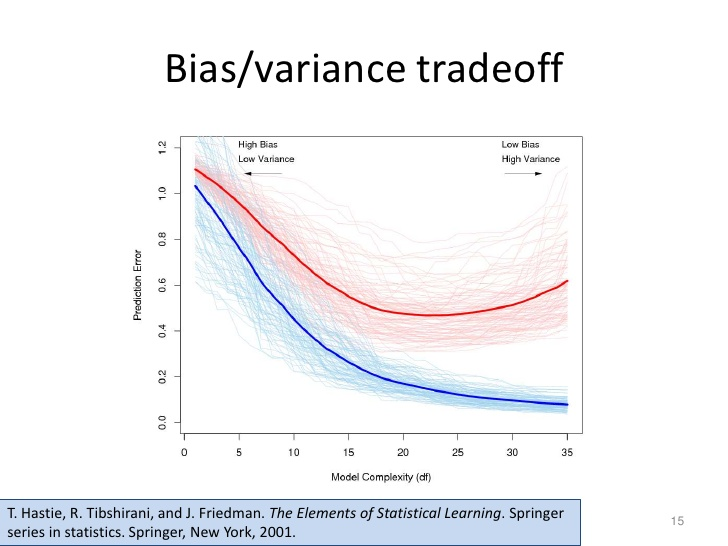
\includegraphics[width=1\textwidth]{art/support-vector-machine-15-728}
        \caption{Overfitting: 
        Prediction error on new data (red curve) versus the empirical prediction error (light blue).
        The empirical prediction error will always decrease as more complicated models are fit (moving right).
        The prediction error on new data, however, will not always decrease and will typically show a local minima.
        \label{fig:bias_variance}}
\end{figure}

Before we proceed, we now need to distinguish between several types of prediction errors.
The population \emph{risk} of a model parametrized by $\theta$, was previously defined as the average loss over all possible data instances, and denoted by $\risk(\theta)$ (\S \ref{sec:m_estimation}).
The empirical risk was defined as the average loss over the observed data points, and denoted by $\riskn(\theta)$.
We now update these definitions to deal with the the $\hyp(x)$ notation of the previous section.
\begin{align}
	\test :=& \expectg{Y,X}{\loss(Y,\hyp(X))}, \label{eq:test_error} \\
	\train :=& \expectn{\loss(y,\hyp(x))} = \frac{1}{n} \sum_i \loss(y_i,\hyp(x_i)),  \label{eq:training_error} \\
	\insample :=& \frac{1}{n} \sum_i \expectg{Y}{\loss(Y,\hyp(x_i))}, \label{eq:in_sample} \\
	\EPE :=& \expectg{\estim{\hyp}_n}{
		\expectg{Y,X}{\loss(Y,\estim{\hyp}_n(X))|\estim{\hyp}_n}
	}.\label{eq:epe}
\end{align}

Eq.(\ref{eq:test_error}) is merely a reformulation of $\risk(\theta)$ from Section~\ref{sec:m_estimation}.
It captures the expected loss, a given predictor, $\hyp(X)$, will incur on average when given new $X$'s and $Y$'s.
This will be the magnitude which will tell us which models perform well, and which do not.
It is known as the \emph{test error} or also as \emph{prediction error}.\marginnote{Test Error}

Eq.(\ref{eq:training_error}) is the reformulation of empirical risk, $\riskn(\theta)$, we have been optimizing in Section~\ref{sec:learning}.
We referred to it as the \emph{empirical risk}, but it is also known as the \emph{train error}.
\marginnote{Train Error}

Eq.(\ref{eq:in_sample}) is the average risk at the observed $x$'s, when given new $Y$'s \footnote{This magnitude should not be unfamiliar: e.g., inference in ANOVA is performed conditional on the $x$'s, which typically stem from a designed experiment.}.
This is the \emph{in sample error}.
\marginnote{In Sample Error}

Eq.(\ref{eq:epe}) is called the \emph{expected prediction error}, i.e., the expected loss when $\hyp$ is also re-learned. 
Put differently: How much would we err when:(1) we are given $n$ new examples $\sample_1$; (2) re-learn $\estim{\hyp}_n$ on $\sample_1$; (3) compute the risk of $\estim{\hyp}_n$ (in the population, not in $\sample_1$.
We emphasize this by writing $\estim{\hyp}_n$ instead of $\hyp$.
$\EPE$ is thus not a property of a particular predictor $\hyp$, but rather of a whole learning algorithm on random samples of size $n$.
It could have also been written as $\risk(algorithm)$, although I have not seen this notation in use.
\marginnote{Expected Prediction Error}


We would like to compare the performance of models based on $\test$, as this will give us an idea on the quality of the prediction on new data. 
Alas, computing $\test$ requires the distribution of $y$ and $x$, while we only have access to the $n$ observed samples.
Can the empirical risk $\train$ estimate the unknown risk $\test$? 
Figure~\ref{fig:bias_variance} suggests it cannot since $\train$ underestimates $\test$.
Why is this?
At an intuitive level: this is because with ERM we learn the $\hyp$ with smallest error in each sample.
It is thus the same as estimating the expected height in a population, by using the minimum in each sample; we will clearly be underestimating the expectation. Then again, there is the hope that we may take this minimum and debias it. 
This is the goal in the next sections.

Before proceeding, we distinguish between two similar tasks: 
\begin{description}
\item[Model Selection] This is the task of selecting between several candidate models.
\item[Model Assessment] This is the task of assessing the prediction error (i.e., the expected loss, the risk) of a given model.
\end{description}



\subsection{Train, Validate, Test}
\label{sec:train_test}
If data is abundant, a trivial, assumption free way to estimate $\test$\footnote{Think: why $\test$ is being estimated, and not $\EPE$ nor $\insample$?}, is to split the data into $3$ sets.
A \emph{training set}, used to learn several competing models.
A \emph{validation set}, used check the performance of the learned models and choose the best performer using some comparison measure. 
A \emph{test set}, used to estimate the risk, as the empirical risk $\train$ will be unbiased to the population risk $\test$.

If there is not enough data for this scheme, keep reading...


\subsection{Unbiased Estimators of the Risk}
\label{sec:risk_estimation}
Under appropriate assumptions, the bias in $\train$ when estimating $\insample$\footnote{In this case, note that it is $\insample$ being estimated, and not $\test$ nor $\EPE$.} can be computed analytically, and accounted for.
The bias $\insample-\train$ is called the \emph{optimism} of the algorithm.\marginnote{Optimism}
Akaike's Information Criterion (AIC), 
the finite sample Corrected AIC (AICc), 
Mallow's Cp (Cp), 
the Bayesian Information Criterion (BIC, aka SBC, aka SBIC), 
the Minimum Description Description Length (MDL), 
Vapnic's Structural Risk Minimization (SRM), 
the Deviance Information Criterion (DIC), 
and the Hannan-Quinn Information Criterion (HQC), 
all try to estimate $\insample$ by correcting for the optimism under different assumptions.\marginnote{Cp, AIC, BIC, MDL, SRM}

The differences, pros, and cons, of each will not be discussed herein. Just remember what they mean when you see them in your favourite software (R!).
They all have in common that you will want the model with the smallest criterion.
But be careful- as they are used for model selection, they are indifferent to scaling, and thus should be not interpreted as the expected prediction error.

\begin{remark}
Not all model selection criteria estimate $\insample$. The Focused Information Criterion (FIC), for example, does not.
\end{remark}





\paragraph{Further Reading}
For a brief review of AIC, BIC, MDL and SRM see Chapter 7 in \citep{hastie_elements_2003}. 
For a more rigorous derivation, see \cite{claeskens_model_2008}.





\subsection{Jackknifing}
\label{sec:jackknife}

If concerned with over fitting, here is a simple algorithm to estimate the prediction error:

\begin{algorithm}[H]
\caption{Jackknife}
\begin{algorithmic}
\For {$i \in 1,\dots,n$}
    \State $\estim{\hyp}^{(i)} \gets$ the learned model with all but the $i$'th observation.
    \State $\loss^{(i)} \gets$ the loss of $\estim{\hyp}^{(i)}$ on the $i$'th observation.
\EndFor
\State \Return the average loss over $\loss^{(i)}$.
\end{algorithmic}
\end{algorithm}

This process is called the \emph{Jackknife}, or \emph{Leave-One-Out--Cross-Validation}. 
This algorithm return an estimator of $\EPE$.
This might be quite surprising: every split uses almost an identical sample, so why would it not estimate $\test$? See Section 7.12 in \cite{hastie_elements_2003} for details..

But wait! We might be able to stabilize the variability of the estimated error in every split, if instead of leaving only a single observation aside, we leave some more. This lead to way to \emph{K-Fold Cross Validation} in the next section.


\subsection{Cross Validation}
\label{sec:cv}

\begin{algorithm}[H]
\caption{Cross Validation}
\begin{algorithmic}
\State Split the data into $\folds$ parts (``folds'').
\For {$\fold \in 1,\dots,\folds$}
    \State $\estim{\hyp}^{(k)} \gets$ the learned model with all \emph{except} the observations in the $\fold$'th fold.
    \State $\loss^{(\fold)} \gets$ the loss average of $\estim{\hyp}^{(\fold)}$ on the observations in the $\fold$'th fold.
\EndFor
\State \Return the average over $\loss^{(\fold)}$ .
\end{algorithmic}
\end{algorithm}

This simple algorithm estimates $\EPE$ without any assumption on the data generating process, and less data than would be required for a ``train-validate-test'' scheme.
Well, as it actually serves for model selection, it should be seen as a ``train-validate'' scheme, without the ``test'' part. It is thus \emph{not} an unbiased estimate of $\EPE$. See Section 7.12 in \cite{hastie_elements_2003} for details.

But wait again! 
The Cross Validation scheme resamples the data \emph{without replacement} to estimate $\EPE$. Could we have sampled it \emph{with} replacement? Yes. This is the idea underlying the \emph{Bootstrapping} scheme.


\subsection{Bootstrapping}
\label{sec:bootstrap}

Here is the simplest version of Bootstrap validation:

\begin{algorithm}[H]
\caption{Bootstrap}
\begin{algorithmic}
\For {$\bootstrap \in 1,\dots,\bootstraps$}
	\State $\sample^\bootstrap \gets$ $n$ randomly selected observations, with replacement, from the original data.
    \State $\estim{\hyp}^{\bootstrap} \gets$ the model learned with  $\sample^\bootstrap$.
    \State $\loss^{\bootstrap} \gets$ the average loss of $\estim{\hyp}^{\bootstrap}$ on the observations in the \emph{original} data.
\EndFor
\State \Return the over of $\loss^{\bootstrap}$ .
\end{algorithmic}
\end{algorithm}

This algorithm is not a good estimator of $\EPE$ as observations play a role both in learning and in validating. 
Several corrections are available. For details see Section 7.11 in \cite{hastie_elements_2003}.

The Bootstrap is a very general scheme, which can be used not only for model validation, but for assessing many of its statistical properties. It is possibly best known when used for hypothesis testing. 
For more on the Bootstrap, see \cite{efron_introduction_1994}.


% Ensembels %
\section{Ensembles}
\label{sec:ensembles}

This section follows the lines of Chapter 8 in \cite{hastie_elements_2003}.

Our inductive bias constrains the hypothesis class so that we do not overfit the data. 
It is overly optimistic to think that nature generates samples in accord with our own inductive bias.
Ensemble learning is a ``meta'' class of algorithms, in which we do not confine ourselves to selecting a single $\hyp$ but rather to selecting (finitely) many, possibly from different classes, and them aggregating them into a single predictor.
This is a very flexible framework that might actually return classifiers that do not belong to any of underlying hypothesis classes. As such, it is an \emph{improper learning} algorithm.\marginnote{Improper Learning}.

One might consider many combinations of hypothesis classes, learning methods and aggregation schemes.
Several celebrated algorithms fall in this class. 



\begin{remark}
As opposed to a \emph{strong learner}, a \emph{weak learner} is a learning algorithm that is only partially optimized for the observed data. 
Some of the above algorithms are motivated by the idea of combining many weak learners from the same $\hypclass$ to return a strong learner. 
Such is the Bagging algorithm. \marginnote{Weak/ Strong Learner}
It has been noted, however, that it is preferable\footnote{Statistically, not necessarily computationally.}  to combine strong learners from different hypothesis classes, then to combine weak learners from the same hypothesis class \cite{gashler_decision_2008}.
\end{remark}




\subsection{Committee Methods}
Considering a set of $\ensembleSize$ candidate learning algorithms, a \emph{committee method} is simply an average of the $\ensembleSize$ predictors:

\begin{algorithm}[H]
\caption{Commitee Methods}
\label{algo:committee}
\begin{algorithmic}
\State For $\ensembleSize$ candidate learning algorithms.
\For{$ \ensembleInd \in 1,\dots,\ensembleSize$}
	\State $\estim{\hyp}^\ensembleInd(x) \gets$ the predictor learned with the $\ensembleInd$'th algorithm.
\EndFor
\State $\bar{\hyp}(x) \gets$ the average of $\estim{\hyp}^\ensembleInd(x)$. 
\State \Return $\bar{\hyp}(x)$
\end{algorithmic}
\end{algorithm}

This concept can be generalized by considering different aggregation schemes. The following (meta-)algorithms are merely different aggregation schemes. Most, if not all, can be seen as minimizers of some posterior expected loss. I.e., they minimize some risk with respect to the posterior probabilities of $\set{\estim{\hyp}^\ensembleInd(x) }_{\ensembleInd=1}^\ensembleSize $.


\subsection{Bayesian Model Averaging}
The idea of \emph{Bayesian model averaging} is that of using the posterior mean as a predictor. 
Computing the posterior mean can be quite a tedious task. 
When dealing with hypotheses from the same parametric class, a more practical approach is that of \emph{inverse BIC weighting}. 
This is justified by that fact that the BIC (\S\ref{sec:risk_estimation}) is approximately proportional to the posterior probability of $\estim{\hyp}^\ensembleInd(x)$.


\begin{algorithm}[H]
\caption{Model Averaging}
\label{algo:model_averaging}
\begin{algorithmic}
\State For $\ensembleSize$ candidate learning algorithms.
\For{$ \ensembleInd \in 1,\dots,\ensembleSize$}
	\State $\estim{\hyp}^\ensembleInd(x) \gets$ the predictor learned with the $\ensembleInd$'th algorithm.
	\State $BIC^\ensembleInd \gets$ the BIC of $\estim{\hyp}^\ensembleInd(x)$.
\EndFor
\State $\bar{\hyp}(x) \gets$ the average of $\estim{\hyp}^\ensembleInd(x)$ inversely weighted by $BIC^\ensembleInd$. 
\State \Return $\bar{\hyp}(x)$
\end{algorithmic}
\end{algorithm}

$BIC$ is used as weights as it approximates the posterior 



\subsection{Stacking}
A simple and powerful (meta-)algorithm by which you train several predictors, and then use their predictions as features for a new predictor. 
A built-in Jackknifing (or Cross Validation) ensures over-fit models are not overweighted.
Here is  stacking example for a continuous $y$:

\begin{algorithm}[H]
\caption{Stacking}
\label{algo:stacking}
\begin{algorithmic}
\State For $\ensembleSize$ candidate learning algorithms.
\For{$ i \in 1,\dots,n$}
	\For{$ \ensembleInd \in 1,\dots \ensembleSize $}
		\State $\estim{\hyp}^{(i)}_\ensembleInd(x) \gets$ the predictor learned with the $\ensembleInd$'th algorithm, and without the $i$'th observation.
	\EndFor
\EndFor
\State $\bar{\hyp}(x_i) \gets$ the OLS prediction using $\set{ \estim{\hyp}^{(i)}_\ensembleInd(x_i)}_{\ensembleInd=1}^\ensembleSize$ as features. 
\State \Return $\bar{\hyp}(x)$
\end{algorithmic}
\end{algorithm}



\subsection{Bootstrap Averaging (Bagging)}

Generates bootstrap samples and averages the learned predictors (see Algorithm~\ref{algo:bagging}). 
While seemingly completely frequentist, the Bootstrap average can be seen as an estimator of the posterior mean for some non-parametric prior.

A \emph{random forrest} is such an algorithm, when CARTs are fitted and averaged. \marginnote{Random Forrest}


\begin{algorithm}[H]
\caption{Bagging}
\label{algo:bagging}
\begin{algorithmic}
\State Choose the number Bootstraps $\bootstraps$.
\For{$ \bootstrap \in 1,\dots,\bootstraps$}
	\State Generate a bootstrap sample of size $n$: $\sample_\bootstrap$.
	\State Learn $\estim{\hyp}(x)_{\bootstrap}$ from $\sample_\bootstrap$.
\EndFor
\State $\bar{\hyp}(x) \gets$ the average of $\estim{\hyp}(x)_{\bootstrap}$.
\State \Return $\bar{\hyp}(x)$
\end{algorithmic}
\end{algorithm}



\subsection{Boosting}
The Boosting algorithm in Section~\ref{sec:boosting} might have the flavour of an Ensemble method, but it should be seen as a regularization scheme. Moving on...






%%%%%%%%% Unsupervised %%%%%%%%%%%

\section{Unsupervised Learning}
\label{sec:unsupervised}

Unlike Supervised Learning, in Unsupervised Learning there is not outcome variable. There is thus no notion of ``right'' and ``wrong''. 
We merely want to learn the joint distribution of the data, $X \in \featureS$, and represent it in some way we can understand. 
Well, maybe ``merely'' is not the right word, as learning the joint distribution of the data means that instead of learning the relation between a set $x$ and another, $y$, we now try to learn the relation between all pairs of variables in $x$, which is clearly more challenging. 

Describing the data via it's joint distribution is the pinnacle, but would require many samples if $x$ has a high dimension (by high we mean $p>3$!). For higher dimensions we need to set more modest goals.

The different goals of unsupervised learning are
\begin{description}
\item[Density Estimation] Estimate the joint density of $x$ over $\featureS$.
\item[Detect high density regions] Find feature combinations which tend to concentrate, hopefully, because the belong to homogenous and interpretable subgroups.
\item[Find low dimensional representations] Find a low dimensional representation of the joint distribution. This allows the learning from realistic sample sizes, and analysis by, e.g., interpretable parameters and visualization.
This goal is discussed in Section~\ref{sec:dim_reduce}.
\end{description}


\paragraph{Relation to Supervised Classification}
Any supervised classification problem can be solved, at least in theory, by solving an unsupervised. 
I.e., estimate the joint distribution within each class, and then classify new observations to the highest density class, via Bayes rule. 
This is known as a \emph{generative} model, as we try to learn the full data generating distribution, unlike the \emph{discriminative} models described above, where the distribution of the features $x$ is of no interest.





\subsection{Density Estimation}
\label{sec:density_estimation}

\subsubsection{Parametric Density Estimation}
Density estimation deals with the learning of the data generating distribution.
If a parametric generative model can be assumed, this collapses to an unsupervised ERM problem. 
Maximum Likelihood estimation being a particularly attractive approach.
If a parametric model cannot be assumed, we fall into the real of non-parametric methods. As we saw for Supervised learning, these typically rely on pooling information from neighbourhoods of $\featureS$.

\subsubsection{Kernel Density Estimation}
\label{sec:kernel_density}

Much like the Kernel Regresson regression, a \naive estimator is the moving average.
A natural generalization, in the spirit of the Nadaraya-Watson smoother (Eq.(\ref{eq:nadaraya_watson})) is the \emph{Parzen} estimate:\marginnote{Parzen Estimate}
\begin{align}
\label{eq:parzen}
	\estim{\pdf}(x):=\frac{1}{n \lambda} \sum_{i=1}^n \kernel_\lambda(x,x_i).
\end{align}

\begin{remark}
If you have been convinced by the use of KNN (\S\ref{sec:knn}) for regression (or classification), there is no reason not to use it for density estimation. It will keep offering the same pros and cons as in KNN regression (or classification).
\end{remark}

As previously stated, these methods may fail when $x$ are high dimensional. We thus recur to other methods.


\subsection{Detect High Density Regions- Cluster Analysis}
When data data is high dimensional so that we cannot perform density estimation, or when we are merely interested in grouping observations, we can still detect high density regions where observations ``clump'' together. Hopefully, into meaningful homogenous groups.
The following methods are thus also known a \emph{bump hunting} or \emph{mode finding}.\marginnote{Bump Hunting}
They are all different heuristic algorithms that return high density regions. Either defined as groups of observations, or as regions in the feature space $\featureS$.

Groups identified are called \emph{clusters}, thus these methods are known as \emph{cluster analysis}, or \emph{data segmentation} methods.

Since these methods are aim at detecting data clustering, they clearly imply the availability of some measure of distance, or similarity, between data points. 


\subsubsection{K Means Clustering}
\label{sec:kmeans}
The idea behind K-means clustering is to find a representative point for each of K clusters, and assign each (unlabeled) data point to one of these clusters. As each cluster has a representative point, this is also a \emph{prototype method}.\marginnote{Prototype Methods}.
The clusters are defined so that they minimize the average distance between all points to the center of the cluster.

In K-means, the clusters are first defined, and then similarities computed. This is thus a \emph{top-down} method.\marginnote{Top Down Clustering}

\begin{algorithm}[H]
\caption{K-Means}
\begin{algorithmic}
\State Choose the number of clusters $K$.
\State Arbitrarily assign points to clusters.
\While {Clusters keep changing}
	\State Compute the cluster centers as the average of their points.
	\State Assign each point to its closest cluster center (in Euclidean distance).
\EndWhile
\State \Return Cluster assignments and means.
\end{algorithmic}
\end{algorithm}



\paragraph{K-Medoids}
If a Euclidean distance is inappropriate for a particular $\featureS$, or that robustness to corrupt observations is required, or that we wish to constrain the cluster centers to be actual observations, then the \emph{K-Medoids} algorithm is an adaptation of K-means that allows this.

\begin{algorithm}[H]
\caption{K-Medoids}
\begin{algorithmic}
\State Choose a similarity metric $\similarity(x_i,x_j)$.
\State Choose the number of clusters $K$.
\State Arbitrarily assign points to clusters.
\While {Clusters keep changing}
	\State Within each cluster, set the center as the data point that minimizes the sum of distances to other points in the cluster.
	\State Assign each point to its closest cluster center (in $\similarity(x_i,x_j)$ distance).
\EndWhile
\State \Return Cluster assignments and centers.
\end{algorithmic}
\end{algorithm}


See Section 14.3.10 in \cite{hastie_elements_2003}.


\subsubsection{Hierarchical Clustering}
\label{sec:hierarchical}
[TODO]


\subsection{Spectral Clustering}
[TODO]


\subsubsection{Association Rules}
\label{sec:association}
Association rules, or \emph{market basket analysis}, or \emph{affinity analysis}, can be seen as approximating the joint distribution with a region-wise constant function (Eq.~\ref{eq:decision_list}).\marginnote{Market Basket Analysis}
Put differently, we want to capture high density regions of the joint distribution of $x$ with by approximating it with a decision-list (not tree).
Learning a decision-list is a computationally impractical problem in general. Association rules are thus typically learned over binary feature spaces $\featureS$, using heuristic optimization schemes.

This type of problems typically occurs in sales analysis, where vendors seek for combinations of products that tend to sell jointly (so that can design the store better, or discount product bundles).

The \emph{Aprioiri} algorithm \cite{agraval_fast_1994}, is an example of such a heuristic search for high density combinations.\marginnote{Apriori Algorithm}







% Generative models %

\section{Generative Models}
\label{sec:generative}

For the mere purpose of making a prediction, we do not need to learn the full data generating distribution $\dist(y,x)$. 
Knowing this distribution, however, does permit to make predictions, via Bayes Theorem: 
$\dist(y|x)=\frac{\dist(y,x)}{\int\dist(y,x)dy}$.
Several supervised and unsupervised methods make use of this relation to make predictions. These are known as \emph{generative models} .
Since the generative distribution serves both in supervised and unsupervised learning, we have dedicated it a section of its own.

\subsection{Density Estimation}
Clearly, the trivial generative model is the density estimation, discussed in Section~\ref{sec:density_estimation}.


\subsection{Fisher's Linear Discriminant Analysis (LDA)}
\label{sec:lda}
The fundamental idea behind Fisher's LDA (sometimes, just LDA) is that for dichotomous $y$'s: $\dist(x|y)$ is multivariate Gaussian, with the same covariance for all $y$.
Estimating $\dist(x|y)$ thus amounts to the estimation of the mean and covariance, which are fairly simple problems that do not require too much data (relatively).

The decision boundaries of this method turn out to be linear in $\featureS$. 
Denoting the distance from the class centers by $\estim{\delta}:=(\estim{\mu}_1-\estim{\mu}_2)$, class thus 2 will be predicted if 
\begin{align}
	x' \estim{\Sigma}^{-1} \estim{\delta} > \frac{1}{2} \estim{\delta}' \estim{\Sigma}^{-1} \estim{\delta}
\end{align}
and class 1 otherwise.


\paragraph{Relation to OLS classification}
Interestingly, the two-class LDA, is the same as a regression classifier from  Section~\ref{sec:regression_classifier} \cite[Eq. 4.11 ]{hastie_elements_2003}.



\subsection{Fisher's Quadratic Discriminant Analysis (QDA)}
If you are uncomfortable with the fixed covariance assumption of LDA, one can relax thus assumption.
This leads to QDA, which is more flexible than LDA, requiring slightly more data, but permitting the learning of a class of quadratic classifiers, and not only linear.






\subsection{\Naive Bayes}
\label{sec:naive_bayes}
In LDA we dealt with the problem of estimating high dimensional distributions by adding the class-wise Gaussianity assumption. As Gaussians as fairly simple to learn from data, if there is any truth to this assumption, our life improved. 
Another life-simplifying assumption, replacing the Gaussianity assumption, is that $\dist(x|y)$ is the product of the margins, i.e., the the features are independent within each class: $\dist(x|y)=\prod_{j=1}^p\dist(x_j|y)$
This greatly simplifies things as estimating the univariate marginal distributions $\dist(x_j|y)$ is a fairly simple problem, which can be done non-parametrically by Kernel smoothing for continuous predictors (\S\ref{sec:kernel}), and simple relative frequencies for discrete predictors. 


%%%%%%%%% Dimension Reduction %%%%%%%%%%%

\section{Dimensionality Reduction}
\label{sec:dim_reduce}
The fundamental idea behind dimensionality reduction is that while $\featureS$ may be high dimensional, thus $\dist(X)$ hard to learn, there is hope that $\x$ does not really vary in the whole space. 
If the mass of $\dist(x)$ is concentrated around some low dimensional manifold $\manifold$, then the original problem might be approximated to learning the distribution of the projection $\dist(X \project \manifold)$ on $\manifold$. 
If $\manifold$ is fairly low dimensional, we may hope to visualize and understand $\dist(X \project \manifold)$ with fairly simple tools.
Dimensionality reduction also reduces the memory required to represent the data. It is thus intimately related to \emph{lossy compression} in information theory.\marginnote{Lossy Compression}

A similar reasoning justifies dimensionality reduction in supervised learning. While $\dist(X)$ might vary in the whole $\featureS$, but there might be only few directions which carry information on $y$. Learning $\dist(Y|X)$ can thus be well approximated by $\dist(Y|X \project \manifold)$.


\begin{remark}
The subspace $\manifold$, which approximates $\dist(X)$ may differ than the one that approximates $\dist(Y|X)$. Despite this, it is still quite common for a supervised learning problem to be preceeded by an unsupervised dimensionality reduction stage.
\end{remark}



\subsection{Dimensionality Reduction In Supervised Learning}
\label{sec:dim_reduce_supervised}
We start with finding a low representation of $x$ that predicts $y$.
This practice has several different motivations. As a regularization device avoiding overfitting, and  as a computational device reducing memory and time complexity. 

\subsubsection{Variable Selection}
A trivial way of reducing the dimension of $x$ is by dropping some of it components. 
Clearly, with $p$ variables, there are $2^p$ possible variable combinations. Searching over all possible variable combinations is called \emph{subset selection}, but is rarely performed in practice due to computational complexity. It more practical to perform a \emph{forward search}, i.e., a greedy search where we insert on variable at a time.\marginnote{Subset Selection}
The search stops when the next variable does not improve the model's accuracy. 
While tempting, measuring the accuracy using the empirical risk will certainly lead to overfitting (see Figure~\ref{fig:bias_variance}).
We can thus drive the search with a CV scheme, but the computational burden might be overwhelming. Using some estimator of $\risk$ auch as AIC, BIC,... is a reasonable and practical way to guide the search.


\begin{algorithm}[H]
\caption{Forward Search}
\begin{algorithmic}
\State Pick your favourite model selection criterion $\estim{\risk}(x)$.
\While{$\estim{\risk}(x)$ keeps getting smaller}
    \State $\estim{\hyp} \gets$ the model with the smallest $\estim{\risk}(x)$ after adding a \emph{single} variable.
\EndWhile
\State \Return $\estim{\risk}(x)$.
\end{algorithmic}
\end{algorithm}



\begin{remark}[Hypothesis Testing Driven Variable Selection]
For a statistician , it is probably very natural to guide a forward search with hypothesis testing. I.e., at each iteration, insert the variable with the most significance. 
Note however, that when interested in good predictions, we might actually gain accuracy by dropping a significant variable. This is a classical bias-variance tradeoff: dropping a true predictor adds bias, but reduces the variance as we have one less parameter to estimate. If the true effect is small, we can gain from this tradeoff. 
This intuition is actually used as a model selection criterion \citep{foster_variable_2004}.
The bottom line is however, that a \textbf{significant variable, does not make it a good predictor.} 
\end{remark}

\subsubsection{LASSO}
We presented the LASSO in Section \ref{sec:lasso} as a regularized ERM problem.
We claimed, without proof, that the $l_1$ regularization in fact performs soft coefficient thresholding. The estimated $\estim{\be}_{LASSO}$ has thus many entries set to zero, acting as a model selection device. 



\subsubsection{Partial Least Squares (PLS) and Canonical Correlation Analysis (CCA)}
\label{sec:pls}
\label{sec:cca}
[TODO]




\subsection{Dimensionality Reduction in Unsupervised Learning}
\label{sec:dim_reduce_unsupervised}

The idea of ERM also applies to unsupervised learning.
If $\hyp(x)$ is low dimensional representation of $x$, mapping it to $\manifold$, we would seek some $\hyp$ that does not incur too much loss, on average. I.e., we seek to minimize $\risk(\hyp)$.

As usual, we do not have access to the data generating process of $x$, so we typically content ourselves with the empirical risk minimization.
In the context of unsupervised learing, the empirical risk is known as the \emph{reconstruction error}.\marginnote{Reconstruction Error}

The building blocks of a supervised learning problem where the loss function $\loss$, the hypothesis class $\hypclass$, a regularization level, and the optimization scheme.
In unsupervised learning, we have similar building blocks. We still have some loss function, regularized or not, penalizing for the poor reconstruction of the data. We can still solve an ERM problem, or replace the optimization by some other learning algorithm. The main difference is in that instead of some low dimensional mapping $\hyp:x \mapsto \estim{y}$, we learn a mapping  $\hyp:x \mapsto \estim{x}$.





\subsubsection{Principal Components Analysis (PCA)}
\label{sec:pca}

PCA is such a basic technique, it has been rediscovered and renamed independently in many fields. 
It can be found under the names of \emph{discrete Karhunen–Loève Transform; Hotteling Transform; Proper Orthogonal Decomposition (POD); Eckart–Young Theorem; Schmidt–Mirsky Theorem;  Empirical Orthogonal Functions; Empirical Eigenfunction Decomposition;  Empirical Component Analysis;  Quasi-Harmonic Modes;  Spectral Decomposition;  Empirical Modal Analysis;} and possibly more\footnote{Wikipedia: \url{http://en.wikipedia.org/wiki/Principal_component_analysis} }.
The many names are quite interesting as they offer an insight into the different problems that led to its (re)discovery.

Starting with an example, consider human height and weight data. 
While clearly two dimensional data, you don't really need both to understand how ``big'' are the people in the data. 
This is because, height and weight vary mostly along a single dimension, which can be interpreted as the ``bigness'' of an individual. 
This is why, physicians use the Body Mass Index (BMI) as an indicator of size, instead of a two-dimensional measurement.
Assume you now wish to give each individual a size score, that is a linear combination of height and weight: PCA does just that. It returns the linear combination that has the most variability, i.e., the combination which best distinguishes between individuals. 


\paragraph{Terminology}
PCA has received much attention. As such, it has rich underlying theory and terminology.
Here are some terms needed to understand PCA outputs:
\begin{itemize}
\item[Principal Components] The linear combinations of the features, which best separate between observations. In our example- the ``bigness'' index of each individual. The first components captures the most variance, the second components, the second most-variance, etc. In terms of $\manifold$, the principal components are an orthogonal basis for $\manifold$.
\item[Scores] Synonymous to Principal Components.
\item[Loadings] The weights of each data point in each principal component. In our example, the importance of the height and weight in constructing the ``bigness'' index.
\end{itemize}


\paragraph{Intuition}
Notice we have currently offered two motivations for PCA: 
(i) Find linear combinations that best distinguish between observations, i.e., maximize variance. 
(ii) Find the linear subspace the bets approximates the data.
The reason these two problems are equivalent, is due to the use of the squares error.
Informally speaking, the data has some total variance. This variance can be decomposed into the part captured in $\manifold$, and the part not captured\footnote{Analogous to $SST=SSR+SSE$ in linear regression.}. 
Since the variance in the data consists of sums of squares, minimizing the distance from $X$ to $\manifold$, is the same as maximizing the variance of $X \project \manifold$, since their sum is fixed.


\paragraph{Mathematics of PCA}

PCA seeks to represent $x$ in the simplest manifold possible: a linear subspace. Thus, $\manifold$ is simply a rank $\rank$ linear subspace in $\mathbb{R}^p$.
A low dimensional representation of the points in the data consists of decoding their low dimensional encoding. 
Since we are dealing with linear spaces, encoding and decoding can be represented with matrices. 
We thus denote the encoding operator by $\encode:\featureS \mapsto \reals^\rank$, a $\rank \times p$ matrix.
We also denote the decoding operator by $\decode:\reals^\rank \mapsto \featureS$ , a $p \times \rank$ matrix. 
Our predictor function ($\hyp$) in this case is $\hyp(x_i)=\decode\encode x_i$.
 
The ERM problem:
\begin{align}
\label{eq:PCA}
	\argmin{\decode,\encode}{\frac{1}{n}\sum_i (x_i-\decode\encode x_i)^2} .
\end{align}

Without proof, it turns out that Eq.(\ref{eq:PCA}) has a closed form solution. 
This solution is typically presented using the Singular Value Decomposition (SVD) of $X$ we now define.\marginnote{SVD}
\begin{definition}[SVD]
Any $n \times p$ matrix $X$, can be decomposed into $X=UDV'$ where 
$U$ is an $n \times p$ orthogonal matrix ($U'U=I_p$); 
$D$ is a $p \times p$ diagonal matrix with diagonal elements $d_1 \geq d_2 \geq \dots \geq d_p$;
$V$ is a $p \times p$ orthogonal matrix ($V'V=I_p$).
\end{definition}

The solution to Eq.(\ref{eq:PCA}) is 
\begin{align}
\label{eq:PCA_solution}
	\estim{\encode} =& V_\rank' \\
	\estim{\decode} =& V_\rank,
\end{align}
where $V_\rank$ are the first $\rank$ columns of $V$ in the Singular Value Decomposition of $X$.





\subsubsection{Kernel Principal Component Analysis (kPCA)}
\label{sec:kpca}

Back to the motivating example from the PCA section (\S\ref{sec:pca}): assume we want to construct a ``bigness'' score, that best separates between individuals, but we no longer constrain it to be a linear function of the height and weight.
We could thus try to solve 
\begin{align}
\label{eq:kpca_wrong}
	\argmax{g}{\covn{g(X)}}
\end{align}
where $\covn{g(X)}$ is the empirical covariance of $g$ applied on each individual, i.e., row-wise on $X$.

Alas, just like in the supervised learning problem, without any constraints on $g$, we might overfit \andor not be able to compute $g$ as optimization is done in a infinite dimensional space. 
We also need to recall that if we allow for a $\rank$ dimensional score, then we have to solve Eq.(\ref{eq:kpca_wrong}) $\rank$ times.
We thus have two matters to attend:
(i) We need to constrain $g$ so that it does not overfit.
(ii) We need the problem to be computable.
This is precisely what kPCA does. 
It turns out, that for a particular class of functions $g$, the optimal $g$'s take a simple form. 
The classes of such $g$'s are known as Reproducing Kernel Hilbert Spaces. They are presented in Appendix~\ref{sec:rkhs}.

The fundamental observation allowing the application of RKHS theory, is that the scores in the PCA problem, actually depend only on the similarities between individuals, as measured by their empirical correlation. 
In kPCA we replace the measure of similarity with some other measure called the \emph{kernel}, chosen from a particular class, and then proceed as if we were solving a PCA problem.


\paragraph{Mathematics of kPCA}
[TODO]


\subsubsection{Sparse Principal Component Analysis (sPCA)}
[TODO]



\subsubsection{Multidimensional Scaling (MDS)}
\label{sec:MDS}
[TODO]


\subsubsection{Graphical Models}
\label{sec:graphical_model}
[TODO]



\subsubsection{Self Organizing Maps (SOM)}
SOMs are aimed at learning low dimensional representations of data useful for clustering. 
As such, they take the form of K-means clustering (\S\ref{sec:kmeans}), but not in the original space $\featureS$ but rather in a low dimensional representation $\manifold$.

For more on SOMs see Section 14.4 in \cite{hastie_elements_2003}. 



\subsubsection{Principal Curves}
[TODO]


\subsubsection{ISOmap}
[TODO]


\subsubsection{LLE}
[TODO]



\subsubsection{Random Projections}
[TODO: Johnson-Lindenstrauss Lemma]



\subsubsection{Compressed Sensing}
\label{sec:compressed_sensing}
[TODO]



\subsubsection{Information Bottleneck}
[TODO]


\begin{remark}[Information Bottleneck and ICA]
[TODO]
\end{remark}

%%%%%%%%% Latent Space Models%%%%%%%%%%%
\section{Latent Space Generative Models}
\label{sec:latent_space}

In the Generative Models section (\S\ref{sec:generative}) we deals with methods for supervised and unsupervised learning that explicitly assume the data generating process.
In this section we pursue this idea, but allow the data generating process to depend on some unobservable quantities-- \emph{latent variables}.
The fundamental idea is that while the data generating distribution may have a complicated form, when we condition on the unobserved variable, the distribution greatly simplifies. 

The latent variables define a \emph{state}. This is why these models are also known as \emph{state space} models. A term coined by \citet{kalman_contributions_1960}.\marginnote{State-Space Models}

\subsection{Mixtures}
[TODO]


\subsection{Regression Switching}
[TODO]



\subsection{Factor Analysis (FA)}
\label{sec:factor_analysis}

Factor Analysis is solved very similarly to PCA (\S\ref{sec:pca}), so that the two are often confused and interchanged. 
FA, however, stems from a rather different motivation than PCA.
In can be seen as a descriptive method using some linear algebra properties.
FA is a generative method, estimable using maximum likelihood. In some cases, the two methods can collapse to the same problem. 
We already know this can happen as we have seen that the Linear Regression problem with Gaussian disturbances can collapse to an OLS problem. 

In FA we assume that the observed $X$'s depend linearly on a set of $\rank$ independent latent (i.e. unobservable) attributes we denote with $\latent$.
The generative model is thus
\begin{align}
\label{eq:factor}
	X=\loadings \latent+\varepsilon
\end{align}
Assuming a generative distribution on $\latent$ and $\varepsilon$, we may try to estimate $\loadings \latent$ by maximum likelihood.
Sadly, recovering the particular latent attributes $\latent$ from $\estim{\loadings\latent}$ is still impossible as there are infinitely many such solutions. To see this, consider an orthogonal \emph{rotation} matrix $\rotation$ ($\rotation' \rotation=I$). For each such $\rotation$: $ \loadings \latent=\loadings \rotation' \rotation \latent = \loadings^* \latent^*$.

The choice of $\rotation$ changes the interpretation of the latent attributes. This is why many researchers find FA an unsatisfactory inference tool.



\paragraph{Terminology}
\begin{description}
\item[Factors] The unobserved attributes $\latent$.
\item[Loadings] The $A$ matrix; the contribution of each attribute to the observed $X$.
\item[Rotation] An orthogonal re-combination of the latent attributes $\latent$ and loadings, which changes the interpretation of the result.
\end{description}

\subsection{Independent Component Analysis (ICA)}
ICA aims at overcoming the non-uniquness of the latent attributes in FA (\S\ref{sec:factor_analysis}).
The fundamental observation is that the non-uniqueness (i.e., non identifiability of $\latent$) stems from the fact that the independent Gaussian distribution is invariant under rotation. I.e. for $\rv \latent \sim \gauss{0,\sigma^2 I}$ is the same as that of $\rotation \rv \latent$. 
By replacing the Gaussianity assumption on the distribution of $\rv \latent$, by some other multivariate distribution, coordinate-wise independent, we can identify $\latent$. 
This is precisely what ICA does. 

\begin{remark}[Blind Source Separation]
ICA is a popular technique in signal processing, where $\latent$ is actually the signal (e.g. sound) produced by several different sources. Recovering $\latent$ is thus recovering the original signals mixing in the recorded $X$. This is known as \emph{blind source separation}.
\end{remark}

\begin{remark}[ICA and FA]
The solutions to the ICA problem can ultimately be seen as a solution to the FA problem with a particular rotation $\rotation$.
Put differently, by the formulation of the ICA problem, implies a specific rotation so that $\latent$ is identifiable. 
\end{remark}

\subsubsection{Mathematics of ICA}
[TODO]

For more on ICA, see \cite{hyvarinen_independent_2000}. 


\subsection{Hidden Markov}
[TODO]


\subsection{Collaborative Filtering}
[TODO]





\newpage

\appendix



\section{Notation}
\label{sec:notation}

In this text we use the following notation conventions:
\begin{description}
\item[$x$] A scalar or vector.
\item[$\x$] A (possibly) vector valued random variable.
\item[$X$] A matrix.
\item[$\x$]  A matrix valued random variable (a random matrix).
\item[$X'$] The matrix transpose of $X$.
\item[$\normII{x}$] The $l_2$ norm of $x$: $\sqrt{\sum_j x_j^2}$.
\item[$\normI{x}$] The $l_1$ norm of $x$: $\sum_j |x_j|$
\item[$\sample$] A data sample.
\item[$\expect{\x}$] The expectation of $\x$.
\item[$\expectn{x}$] The empirical expectation (average) of the vector $x$.
\item[$\cov{\x}$] The covariance matrix of $\x$: $\expect{(\x-\expect{\x})(\x-\expect{\x})'}$.
\item[$\covn{x}$] The empirical covariance matrix of x: $\expectn{(x-\expectn{x})(x-\expectn{x})'}$.
\item[$\cdf{x}{t}$] The CDF of $\x$ at $t$.
\item[$\icdf{x}{\al}$] The inverse CDF at $\al$ (the quantile function).
\item[$\cdfn{x}{t}$] The empirical CDF of data vector $x$.
\item[$\icdfn{x}{\al}$] The empirical $\al$ quantile of the data vector $x$.
\item[$\x \sim \dist$]  The random variable $\x$ is $\dist$ distributed. 
\item[$\pdf(x)$] The density function of $\dist$ at $x$.
\item[$\gauss{\mu,\sigma^2}$] The univariate Gaussian distribution with mean $\mu$ and variance $\sigma^2$.
\item[$\gauss{\mu,\Sigma}$] The multivariate Gaussian distribution with mean vector $\mu$ and covariance matrix $\Sigma$.
\item[$\lik(\theta)$] The likelihood function at $\theta$.
\item[$\loglik(\theta)$] The log likelihood function at $\theta$.
\item[$\loss(x,\theta)$] The loss function of $\theta$ at $x$.
\item[$\risk(\theta)$]  The risk at $\theta$.
\item[$\riskn(\theta)$] The empirical risk at $\theta$.
\item[$\hyp(x)$] A prediction (hypothesis) at $x$.
\item[$\hypclass$] The class of all hypotheses $\hyp$.
\item[$\plane$] A hyperplane.
\item[$\categories$] A set of categories. 
\item[$\positive{t}$] The positive part of $t$.
\item[$\kernel(x,y)$] A kernel function evaluated at $(x,y)$.
\item[$\indicator{A}$] The indicator function of the set $A$.
\item[$\manifold$] A manifold.
\item[$\project$] A projection operator.

\end{description}



\section{The Kernel Trick and Reproducing Kernel Hilbert Spaces (RKHS)}
\label{sec:rkhs}

Think of smoothing splines (\S\ref{sec:smoothing_splines});
It was quite magical that without constraining the hypothesis class $\hypclass$, the ERM problem in Eq.(\ref{eq:smoothing_spline}) has a finite dimensional closed form solution.
The property of an infinite dimensional problem having a solution in a finite dimensional space is known as the \emph{kernel property} in the machine learning literature.\marginnote{Kernel Property}
We with to generalize this observation and ask- which problems have the kernel property?
Stating the general optimization problem:
\begin{align}
\label{eq:rkhs}
	\argmin{\hyp}{\frac{1}{n} \sum_i \loss(y_i,\hyp(x_i)) + \lambda J(\hyp) }
\end{align}
The problem is then- what type of penalties $J(\hyp)$ will return simple solutions to Eq.(\ref{eq:rkhs}).
The answer is: function that belong to =\emph{Reproducing Kernel Hilbert Space} function spaces. 
RKHS's are denoted by $\rkhs$.
They include many functions, but they are a rather ``small'' subset of the space of all possible functions.
These spaces, and the functions therein, are defined by another function called a \emph{Kernel} denoted by $\kernel$. 
Choosing a particular kernel defines the space and the functions therein.
Choosing a particular kernel, also defines the form of $J$ in Eq.(\ref{eq:rkhs}).
Put differently: for any choice of a kernel $\kernel$, there is a particular $J(\hyp)$ for which the solution of Eq.(\ref{eq:rkhs}) will be a function in $\rkhs$ and will be easily computable. 


\subsection{Mathematics of RKHS}
We now show how choosing a kernel $\kernel$ defines a space $\rkhs$, and a penalty $J(\hyp)$.

A kernel is a non-negative symmetric function of two arguments: $\kernel(x,y): \reals^p \times \reals^p \mapsto \reals_+$.
By fixing $y$, $\kernel(x,y)$ is a function with a single argument $x \mapsto \kernel(x,y)$.
$\rkhs$ is merely the space of functions of $x$, spanned at given $y$'s: 
\begin{align}
\label{eq:rkhs_span}
	\hyp(x):\sum_m \al_m \kernel(x,y_m)
\end{align} 

From linear algebra, you may know that positive definite matrices be diagonalized. 
This analogy carries to $\kernel$, which admits an eigen-expansion: 
\begin{align}
\label{eq:rkhs_eigen}
	\kernel(x,y)=\sum_{i=1}^\infty \gamma_i \phi(x) \phi(y)
\end{align}
Using Eqs.(\ref{eq:rkhs_eigen}) and (\ref{eq:rkhs_span}) we can thus expand elements $f$ of $\rkhs$: 
\begin{align}
	\hyp(x)=\sum_{i=1}^\infty c_i \phi(x)
\end{align}
where $c_i=\gamma_i \sum_m \alpha_m \phi(y)$.
We also define a norm $\normrkhs{\hyp}^2$ in this space, which is induced by $\kernel$:
\begin{align}
\label{eq:rkhs_norm}
	\normrkhs{\hyp}^2 := \sum_{i=1}^\infty \frac{c_i^2}{\gamma_i}
\end{align}

The penalty $J(\hyp)$ in Eq.(\ref{eq:rkhs}), is simply be $\normrkhs{\hyp}^2$.
The $\hyp$'s that solve Eq.(\ref{eq:rkhs}) are guaranteed to have a simple form. They reside in an $n$ dimensional linear function space \citep{wahba_spline_1990}:
\begin{align}
	\hyp(x)=\sum_{i=1}^n \al_i \kernel(x,x_i)
\end{align}

The functions $\kernel(x,x_i)$ can be seen as a basis to the solution space. 
The good news continue! Being only $n$ dimensional, the norms of these $\hyp$'s, do not require integration but rather only finite summation:
\begin{align}
	\normrkhs{\hyp}^2=\sum_{i=1}^n \sum_{j=1}^n \kernel(x_i,x_j) \al_i \al_{j} := \al' K \al.
\end{align}

Adding the above results, we can restate Eq.(\ref{eq:rkhs}) and say that when fixing $\kernel$ and using the appropriate $J$, we only need to solve: 
\begin{align}	
\label{eq:rkhs_simple}
		\argmin{\al}{\frac{1}{n} \sum_i \loss(y_i-K_i \alpha) + \lambda \al' K \al }
\end{align}
which is a quadratic programming problem over an $n$ dimensional linear space, easily solvable with numeric routines.


\subsection{The Bayesian View of RKHS}
Just as the ridge regression (\S\ref{sec:ridge}) has a Bayesian interpretation, so does the kernel trick.
Informally, the functions solving Eq.(\ref{eq:rkhs}) can be seen as the posterior mode if our prior beliefs postulate that the function we are trying to recover is a Gaussian zero-mean process with covariance given by $\kernel$.
This view suggests the intuition that the regularization introduced by $J(\hyp)$ shrinks the estimated $\hyp$ towards a smoother function. At an extreme, where $\lambda\to\infty$, we will recover a constant function, since the the mode of our Gaussian process prior is at the origin of $\rkhs$.

%%%%%%%%% Algorithms %%%%%%%%%%%
\newpage

\listofalgorithms
\addcontentsline{toc}{section}{List of Algorithms}


%%%%%%%%% Bibliography %%%%%%%%%%%
\newpage

\addcontentsline{toc}{section}{Bibliography}

\bibliographystyle{abbrvnat}
\bibliography{Intro2MachineLearning}


\end{document}